%% LyX 2.1.4 created this file.  For more info, see http://www.lyx.org/.
%% Do not edit unless you really know what you are doing.
\documentclass[10pt,english]{article}
\usepackage[T1]{fontenc}
\usepackage[latin9]{inputenc}
\usepackage{geometry}
\geometry{verbose,tmargin=2cm,bmargin=2cm,lmargin=2cm,rmargin=2cm}
\usepackage{color}
\usepackage{babel}
\usepackage{float}
\usepackage{amsmath}
\usepackage{graphicx}
\usepackage{esint}
\usepackage[unicode=true,
 bookmarks=true,bookmarksnumbered=true,bookmarksopen=false,
 breaklinks=false,pdfborder={0 0 0},backref=false,colorlinks=true]
 {hyperref}
\usepackage{breakurl}

\makeatletter
%%%%%%%%%%%%%%%%%%%%%%%%%%%%%% User specified LaTeX commands.
\renewcommand\[{\begin{equation}}
\renewcommand\]{\end{equation}}

\makeatother

\begin{document}

\title{Adding Sensitivity to 21cm Inteferometric Probes of Reionization}

\maketitle

\section{Introduction}

The epoch of reionization represents the last key stage of the universe's
early evolution. Specifically, study of this event marks the intersection
of early cosmology and astrophysics. Understanding this event is important
not only as a scientific goal of its own, but also potentially provides
crucial information to fundamental nature of inflation, neutrino mass
and phenonmenology of the first stars and galaxies alike. 

Arguably the most promising observational probe of the epoch of reionization
comes from measurement of the ``spin-flip'' transition of neutral
hydrogen of characteristic wavelength 21cm. While probes relying on
emission and scattering of free electrons are limited to the lower
redshifts after the completion of reionization, the 21cm line directly
probes the abundance and distribution of neutral hydrogen, and thus
would potentially shed light on the entire cosmic dawn. Thus radio
interferometry techniques to measure the 21cm power spectrum has been
a top priority in astronomy. Cuurrent generation instruments include
the Precision Array for Probing the Epoch of Reionization (PAPER),
Murchison Widefield Array (MWA), Low Frequency Array (LOFAR), and
next generation instruments such as the Hydrogen Epoch of Reionization
Array (HERA) and the Square Kilometer Array Low (SKA low) are under
construction. 

One of the main challenges of interferometric observations of cosmic
21cm line is the foreground contaminations. Both sources within our
galaxy, and to a lesser extent sources outside of our galaxy emit
radio contaminations up to five orders of magnitude higher than the
reionization signal. There are two common methods to deal with the
foreground contamination. In the first, individual sources are identified
and removed, sometimes called the foreground removal technique. The
other technique, commonly refered to as foreground avoidance, makes
use of the fact that most foreground contamination is a smooth spectrum,
and thus is contrained to a Fourier domain ``foreground wedge''.
The main challenge of using the latter technique is the sensitivity,
or the signal to noise ratio. This is the motivation for the design
of the maximum redundancy arrays such as MWA, PAPER, and HERA. While
traditional imaging arrays such as the Very Large Array (VLA) focus
on Fourier mode uv coverage, the redundant arrays have many tightly
packed antennas at equal spacing. Since baselines of the same length
and orientation measure the same Fourier modes on the sky, the maximum
redundancy arrays is able to increase the signal to noise ratio of
the Fourier mode in question. Ali2015 provided the newest upper limit
to the power spectrum measurements with the PAPER-64 data. Some models
expect that the sensitivity required for detection is a factor of
2 away. 

The earth's rotation causes the baseline to sweep through different
areas of the sky during the day. This effect is used extensively to
improve uv coverage in imaging with minimum redundancy arrays. In
a redundant array, baselines that are slightly different rotate into
each other at a time delay. Here we present a method to improve the
sensitivity of the maximum redundancy arrays by considering the uv
redundancy of different baselines at a time lag. In section 2 we present
the basic search algorithm for this time delay. In section 3 we present
a necessary correction and comparison with simulated data. 


\section{Time delayed redundancy}

Baselines of the same length and orientation are traditionally called
``redundant baselines'', because they measure the same Fourier mode
in the sky. In order to eliminate confusion, we shall introduce slightly
different terminology. We'll call baselines that are the same length
and orientation ``equivalent baselines''. Two equivalent baselines
will be redundant with each other simultaneously. Some non-equivalent
baselines can also be redundant if their respected time series is
shifted with respect to one another by a certain delay. We call the
latter ``near equivalent baselines''. It is our goal to a) identify
the near equivalent baselines that give good delayed redundancy, b)
to find this delay for a given pair of baselines, and c) to quantify
the sensitivity improvement associated with cross multiplying such
a pair of nonequivalent baselines. 


\subsection{Cross multiplication of near redundant data}

To begin, we first derive theoretical expectations of cross correlation
of two near-equivalent baselines. Given a point source on the sky,
each baseline measures a track of the source in uv plane. We identify
redundancy of near equivalent baselines for that point source as crossings
of the tracks. Since processed data are measured at discrete time
intervals (in lst-binned PAPER-64 data it's 42.9 seconds ), we do
not have exact overlap of two data points in uv space. We thus need
to find a way to cross multiply data points that are separated by
a short distance in uv space and recover the power spectrum. 

We take the visibility as 
\[
\begin{aligned}V_{\nu}(b) & =\int d\Omega A(\hat{r})I(\hat{r})\exp\left[-2\pi i\frac{\nu}{c}b\cdot\hat{r}\right],\\
 & \approx\frac{2k_{B}}{\lambda^{2}}\int d\Omega A(\hat{r})T(\hat{r})\exp\left[-2\pi i\frac{\nu}{c}b\cdot\hat{r}\right],\\
 & =\frac{2k_{B}}{\lambda^{2}}\int\frac{d^{3}r}{X^{2}Y}A(r)T(r)e^{-ikr}.
\end{aligned}
\]
Here $\lambda$ is a mean wavelength, $\boldsymbol{b}$ is the baseline
length, $\hat{\boldsymbol{r}}$ is a direction in the sky, $A$ is
the beam, and $I$ is the intensity, which has been related to $T$,
the brightness temperature. In the last line $(r_{x},r_{y},r_{z})=(Xl,Xm,Y\nu)$,
and $(Xk_{x},Xk_{y},Yk_{z})=2\pi(u,v,\eta)$. 

We define the delay transformed visibility:
\[
\begin{aligned}V(b) & =\int d\nu V_{\nu}(b)\exp\left[-2\pi i\nu\eta\right],\\
 & =\frac{2k_{B}}{\lambda^{2}}\int d\Omega d\nu A(\hat{r},\nu)T(\hat{r},\nu)\exp\left[-2\pi i\left(\frac{\nu}{c}b\cdot\hat{r}+\nu\eta\right)\right]
\end{aligned}
\]


\textbackslash{}The beam reception pattern $A$ is dimensionless,
normalized to 1 at its peak (zenith), and we assume it to be the same
for all baselines. We introduce the Fourier temperature and window
function

\[
\begin{aligned}\tilde{T}(k) & =\int\frac{d^{3}r}{X^{2}Y}T(r)e^{-ikr},\\
W(k) & =\int d^{3}rA(r)e^{-ikr}.
\end{aligned}
\]
By the convolution theorem, we have
\[
\begin{aligned}\tilde{V}(k) & \approx\frac{2k_{B}}{\lambda^{2}}\int\frac{d^{3}r}{X^{2}Y}A(r)T(r)e^{-ikr},\\
 & =\frac{2k_{B}}{\lambda^{2}}\frac{1}{(2\pi)^{3}}\int d^{3}k_{1}W(k_{1})\tilde{T}(k+k_{1}).
\end{aligned}
\]
With implicit bounds of integrals from $-\infty$ to $\infty$, we
have
\begin{equation}
\begin{aligned}\langle\tilde{V}^{*}(k-k_{r})\tilde{V}(k)\rangle & =\left(\frac{2k_{B}}{\lambda^{2}}\right)^{2}\frac{1}{(2\pi)^{6}}\int dk_{1}dk_{2}W^{*}(k_{1})W(k_{2})\langle T^{*}(k+k_{1}-k_{r})T(k+k_{2})\rangle,\\
 & =\left(\frac{2k_{B}}{\lambda^{2}}\right)^{2}\frac{1}{(2\pi)^{6}}\int dk_{1}dk_{2}W^{*}(k_{1})W(k_{2})\delta_{D}(k_{2}-k_{1}-k_{r})\hat{P_{21}}(k+k_{2}),\\
 & \approx\left(\frac{2k_{B}}{\lambda^{2}}\right)^{2}\frac{\hat{P_{21}}(k)}{(2\pi)^{6}}\int dk_{1}W^{*}(k_{1})W(k_{1}+k_{r}),\\
 & =\left(\frac{2k_{B}}{\lambda^{2}}\right)^{2}\frac{\hat{P_{21}}(k)}{(2\pi)^{3}}\int d^{3}r|A(r)|^{2}e^{-ik_{r}r},\\
 & =\left(\frac{2k_{B}}{\lambda^{2}}\right)^{2}\frac{\hat{P_{21}}(k)}{(2\pi)^{3}}\int d^{3}r|a(r)\phi(r_{z})|^{2}e^{-ik_{r}r}
\end{aligned}
\label{eq:(7)}
\end{equation}
where the first to second line follows from assumption of Gaussian
random sky, and the second to third line follows from the assumption
that the 3D power spectrum varies neglegibly over the region of interest
so that $\hat{P_{21}}(k+k_{2})\approx\hat{P_{21}}(k)$. In the last
line we have separated the 2D spatial beam patter from the frequency
bandpass $\phi$. So in conclusion the cross correlation of visibilities
seperated by $\Delta u$ apart in uv space is proportional to the
power spectrum times the Fourier transform of the beam pattern squared. 

\begin{figure}[H]
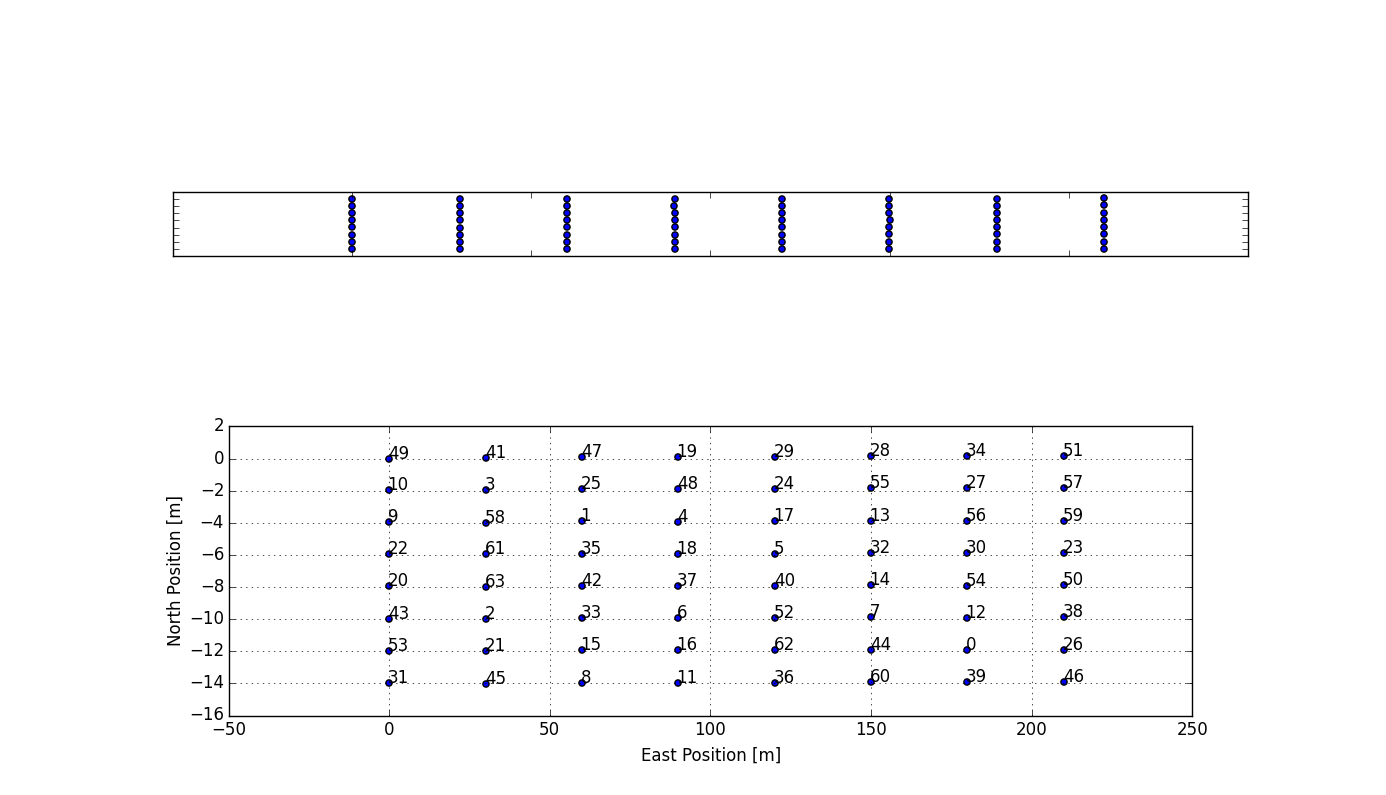
\includegraphics[scale=0.5]{64layout}

\caption{The PAPER 64 layout. Top panel shows the antenna positions drawn to
scale, bottom panel show the antenna labels and distances. }
\end{figure}


We shall use the 64-antenna PAPER array to demonstrate. The PAPER
64 array is located in the Karoo desert in South Africa (30:43:17.5
S, 21:25:41.8 E). The layout pattern with antenna labels are show
in Fig. 1. I show denote a baseline with the antconfigWe see the antenna
spacing in North-South directions are comparatively close (4m), so
that baselines such as 0\_44 and 0\_7 are very close to equivalent. 


\section{Implementation}

An example of rotation tracks is shown in the uv plane below

\begin{figure}[H]
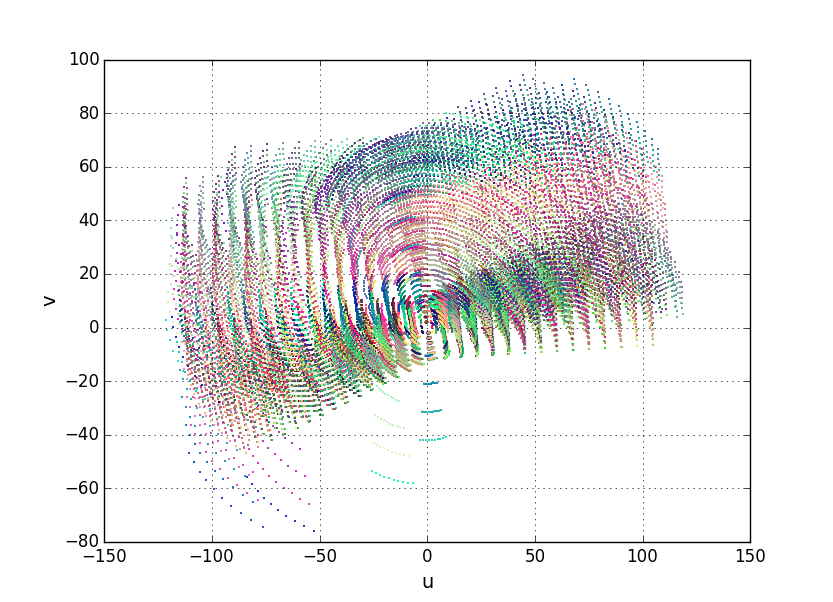
\includegraphics[scale=0.5]{tracks}

\caption{The PAPER 64 layout. Top panel shows the antenna positions drawn to
scale, bottom panel show the antenna labels and distances. }
\end{figure}


The beam squared and its Fourier transform are given as

\begin{figure}[H]
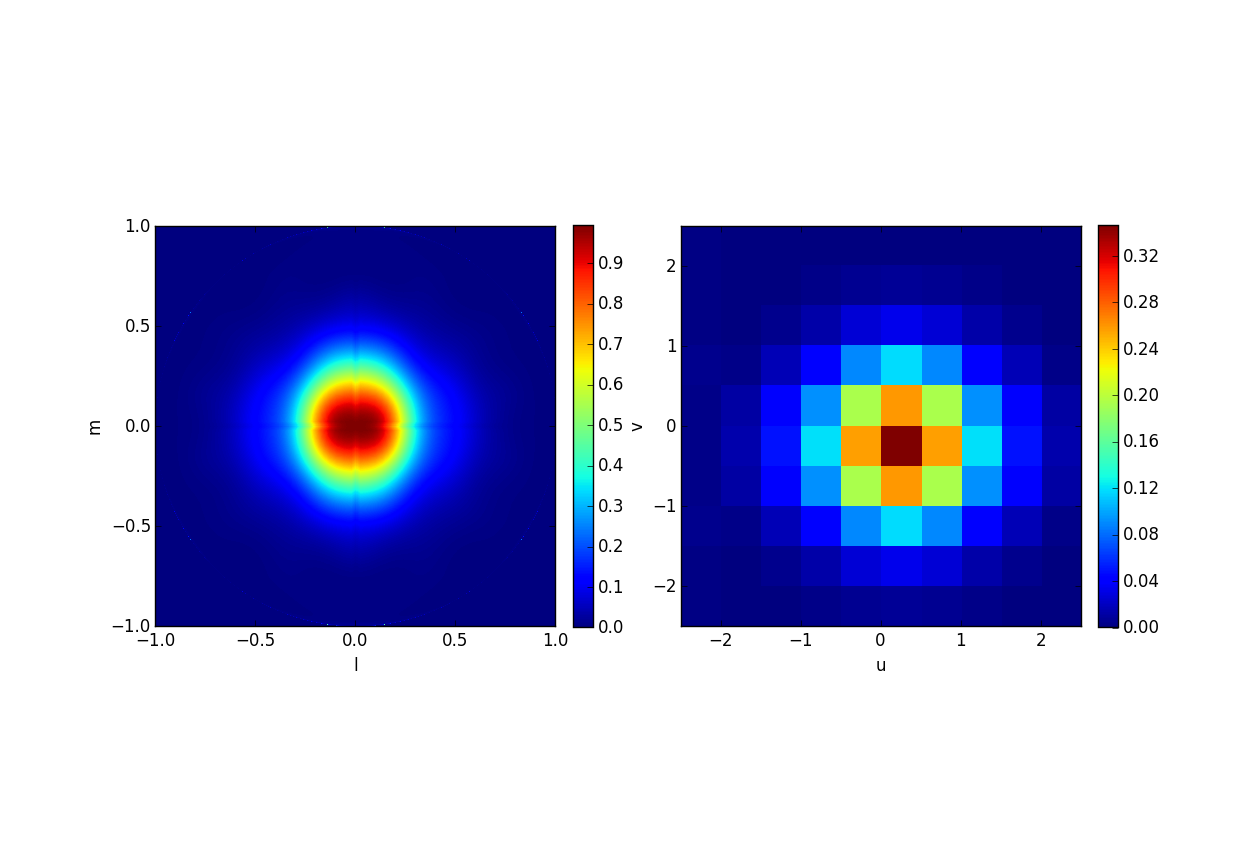
\includegraphics[scale=0.4]{64beam}

\caption{The PAPER 64 layout. Top panel shows the antenna positions drawn to
scale, bottom panel show the antenna labels and distances. }
\end{figure}

\end{document}
